\begin{multicols}{2}
    [
        The six different combinations of alignment- and tree searching-methods resulted in four different trees
        for the major taxa of Isoptera, Cryptocercus punctulatus, Blattidae and Blaberoidea with the Mantoida
        as the outgroup (figure 2). All trees aligned using the Muscle-algorithm resulted in the same topologies
        for the major taxa.
    ]
    \lipsum[2-6]
\end{multicols}

\begin{figure}[H]
    \centering
    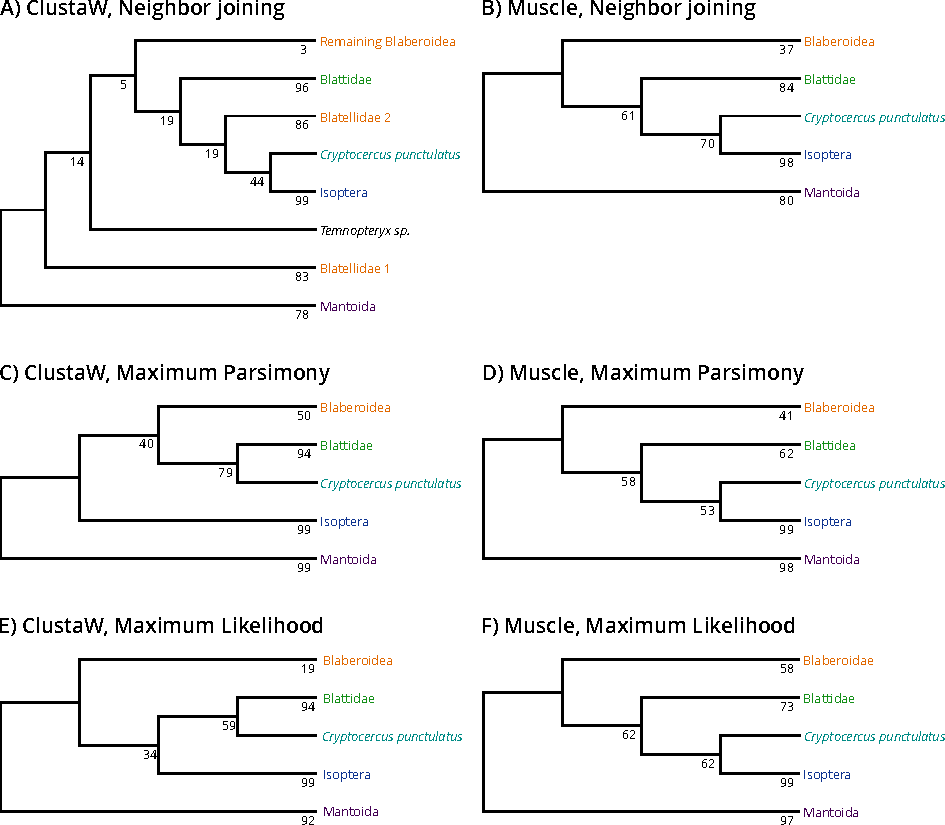
\includegraphics[scale=1]{images/collapsed_trees.pdf}
    \vspace{0.5cm}
    \mycaption{Bold short title}{of an example figure \lipsum[2].} 
    \label{fig:majortaxa}
\end{figure}